% -*- coding: utf-8 -*-
%-------------------------designed by zcf--------------
\documentclass[UTF8,a4paper,10pt]{ctexart}
\usepackage[left=3.17cm, right=3.17cm, top=2.74cm, bottom=2.74cm]{geometry}
\usepackage{amsmath}
\usepackage{graphicx,subfig}
\usepackage{float}
\usepackage{cite}
\usepackage{caption}
\usepackage{enumerate}
\usepackage{booktabs} %表格
\usepackage{multirow}
\newcommand{\tabincell}[2]{\begin{tabular}{@{}#1@{}}#2\end{tabular}}  %表格强制换行
%-------------------------字体设置--------------
% \usepackage{times} 
\usepackage{ctex}
\setCJKmainfont[ItalicFont=Noto Sans CJK SC Bold, BoldFont=Noto Serif CJK SC Black]{Noto Serif CJK SC}
\newcommand{\yihao}{\fontsize{26pt}{36pt}\selectfont}           % 一号, 1.4 倍行距
\newcommand{\erhao}{\fontsize{22pt}{28pt}\selectfont}          % 二号, 1.25倍行距
\newcommand{\xiaoer}{\fontsize{18pt}{18pt}\selectfont}          % 小二, 单倍行距
\newcommand{\sanhao}{\fontsize{16pt}{24pt}\selectfont}  %三号字
\newcommand{\xiaosan}{\fontsize{15pt}{22pt}\selectfont}        % 小三, 1.5倍行距
\newcommand{\sihao}{\fontsize{14pt}{21pt}\selectfont}            % 四号, 1.5 倍行距
\newcommand{\banxiaosi}{\fontsize{13pt}{19.5pt}\selectfont}    % 半小四, 1.5倍行距
\newcommand{\xiaosi}{\fontsize{12pt}{18pt}\selectfont}            % 小四, 1.5倍行距
\newcommand{\dawuhao}{\fontsize{11pt}{11pt}\selectfont}       % 大五号, 单倍行距
\newcommand{\wuhao}{\fontsize{10.5pt}{15.75pt}\selectfont}    % 五号, 单倍行距
%-------------------------章节名----------------
\usepackage{ctexcap} 
\CTEXsetup[name={,、},number={ \chinese{section}}]{section}
\CTEXsetup[name={(,)},number={\chinese{subsection}}]{subsection}
\CTEXsetup[name={,.},number={\arabic{subsubsection}}]{subsubsection}
%-------------------------页眉页脚--------------
\usepackage{fancyhdr}
\pagestyle{fancy}
\lhead{\kaishu \leftmark}
% \chead{}
\rhead{\kaishu 编译系统原理实验报告}%加粗\bfseries 
\lfoot{}
\cfoot{\thepage}
\rfoot{}
\renewcommand{\headrulewidth}{0.1pt}  
\renewcommand{\footrulewidth}{0pt}%去掉横线
\newcommand{\HRule}{\rule{\linewidth}{0.5mm}}%标题横线
\newcommand{\HRulegrossa}{\rule{\linewidth}{1.2mm}}
%-----------------------伪代码------------------
\usepackage{algorithm}  
\usepackage{algorithmicx}  
\usepackage{algpseudocode}  
\floatname{algorithm}{Algorithm}  
\renewcommand{\algorithmicrequire}{\textbf{Input:}}  
\renewcommand{\algorithmicensure}{\textbf{Output:}} 
\usepackage{lipsum}  
\makeatletter
\newenvironment{breakablealgorithm}
  {% \begin{breakablealgorithm}
  \begin{center}
     \refstepcounter{algorithm}% New algorithm
     \hrule height.8pt depth0pt \kern2pt% \@fs@pre for \@fs@ruled
     \renewcommand{\caption}[2][\relax]{% Make a new \caption
      {\raggedright\textbf{\ALG@name~\thealgorithm} ##2\par}%
      \ifx\relax##1\relax % #1 is \relax
         \addcontentsline{loa}{algorithm}{\protect\numberline{\thealgorithm}##2}%
      \else % #1 is not \relax
         \addcontentsline{loa}{algorithm}{\protect\numberline{\thealgorithm}##1}%
      \fi
      \kern2pt\hrule\kern2pt
     }
  }{% \end{breakablealgorithm}
     \kern2pt\hrule\relax% \@fs@post for \@fs@ruled
  \end{center}
  }
\makeatother
%------------------------代码-------------------
\usepackage{xcolor} 
\usepackage{listings} 
\usepackage{graphicx}
\lstset{ 
breaklines,%自动换行
basicstyle=\small,
escapeinside=``,
keywordstyle=\color{ blue!70} \bfseries,
commentstyle=\color{red!50!green!50!blue!50},% 
stringstyle=\ttfamily,% 
extendedchars=false,% 
linewidth=\textwidth,% 
numbers=left,% 
numberstyle=\tiny \color{blue!50},% 
frame=trbl% 
rulesepcolor= \color{ red!20!green!20!blue!20} 
}
%------------超链接----------
\usepackage[colorlinks,linkcolor=black,anchorcolor=blue]{hyperref}
%------------------------TODO-------------------
\usepackage{enumitem,amssymb}
\newlist{todolist}{itemize}{2}
\setlist[todolist]{label=$\square$}
% for check symbol 
\usepackage{pifont}
\newcommand{\cmark}{\ding{51}}%
\newcommand{\xmark}{\ding{55}}%
\newcommand{\done}{\rlap{$\square$}{\raisebox{2pt}{\large\hspace{1pt}\cmark}}\hspace{-2.5pt}}
\newcommand{\wontfix}{\rlap{$\square$}{\large\hspace{1pt}\xmark}}
%------------------------水印-------------------
\usepackage{tikz}
\usepackage{xcolor}
\usepackage{eso-pic}
\usepackage{verbatim}

\newcommand{\watermark}[3]{\AddToShipoutPictureBG{
\parbox[b][\paperheight]{\paperwidth}{
\vfill%
\centering%
\tikz[remember picture, overlay]%
  \node [rotate = #1, scale = #2] at (current page.center)%
    {\textcolor{gray!80!cyan!30!magenta!30}{#3}};
\vfill}}}

%———————————————————————————————————————————正文
%----------------------------------------------
\begin{document}
\begin{titlepage}
    \begin{center}
    
\includegraphics[width=0.8\textwidth]{NKU.png}\\[1cm]    
    \textsc{\Huge \kaishu{\textbf{南\ \ \ \ \ \ 开\ \ \ \ \ \ 大\ \ \ \ \ \ 学}} }\\[0.9cm]
    \textsc{\huge \kaishu{\textbf{网\ \ 络\ \ 空\ \ 间\ \ 安\ \ 全\ \ 学\ \ 院}}}\\[0.5cm]
    \textsc{\Large \textbf{编译系统原理实验报告}}\\[0.8cm]
    \HRule \\[0.9cm]
    { \LARGE \bfseries Lab0 \ 了解编译器}\\[0.4cm]
    \HRule \\[2.0cm]
    \centering
    \textsc{\LARGE \kaishu{张丛\ \ \ 刘国民 }}\\[0.5cm]
    \textsc{\LARGE \kaishu{年级\ :\ 2021级}}\\[0.5cm]
    \textsc{\LARGE \kaishu{专业\ :\ 信息安全}}\\[0.5cm]
    \textsc{\LARGE \kaishu{指导教师\ :\ 王刚}}\\[0.5cm]
    \vfill
    {\Large \today}
    \end{center}
\end{titlepage}
%-------------摘------要--------------
\newpage
\thispagestyle{empty}
\renewcommand{\abstractname}{\kaishu \sihao \textbf{摘要}}
    \begin{abstract}
        % \noindent  %顶格
本次实验以阶乘程序为例,详细分析了由C/C++语言源代码生成可执行文件的具体过程,总体上可分为预处理、编译、汇编和链接四个部分。同时还编写和分析了LLVM IR程序,熟悉了编译过程中所使用的中间语言。本次实验第一节和第二节由张丛同学负责,第三至五节由刘国民同学负责。
        \textbf{\\ 关键字:编译;LLVM;GCC}\textbf{} \\\ \\\
    \end{abstract}
%----------------------------------------------------------------
\tableofcontents
%----------------------------------------------------------------
\newpage
\watermark{60}{10}{NKU}
\setcounter{page}{1}
\section{正文}



%——————————————————————————————————————
\subsection{第一节 \ \ 预处理器}
预处理阶段会处理预编译指令,包括绝大多数的\verb|#|开头的指令,如 \verb|#|include、\verb|#|define、\verb|#|if等等,对 \verb|#|include 指令会替换对应的头文件,对 \verb|#|define 的宏命令会直接替换相应内容,同时会删除注释,添加行号和文件名标识。


若是我们自己创建的头文件则需将<>替换成"",此时系统会先从项目文件夹中寻找是否存在相应的头文件,其次会从库文件中寻找,再否则会抛出错误。

如图\ref{fig:1}所示的cpp文件仅有15行代码
\begin{figure}[H]
    \centering
    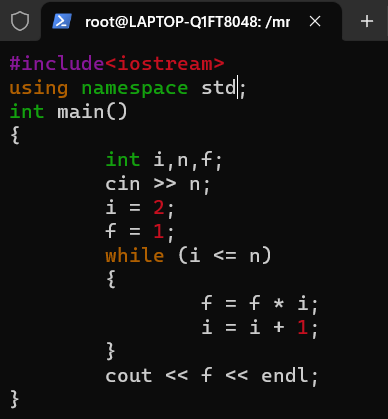
\includegraphics[width=0.5\textwidth]{imgs/cppcode.png}
    \caption{cpp代码}
    \label{fig:1}
\end{figure}

在经过以下命令后得到预处理文件:
\begin{lstlisting}[frame=trbl]
  g++ main.cpp -E -o main.i
\end{lstlisting}\par

如图\ref{fig:2},得到的预处理文件总共有32268行,远多于源文件
\begin{figure}[H]
    \centering
    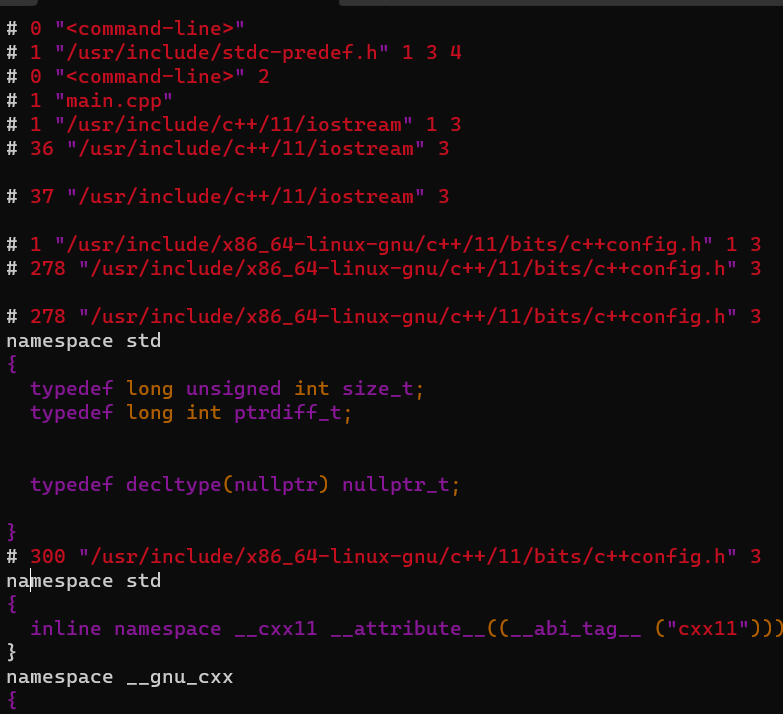
\includegraphics[width=0.5\textwidth,height=0.5\textwidth]{imgs/maini.png}
    \caption{main.i代码}
    \label{fig:2}
\end{figure}
就图\ref{fig:2}来说,预处理器预处理了系统头文件和std命名空间的模板结构等等。


%——————————————————————————————————————
\subsection{第二节 \ \ 编译器}
编译器进行了六个过程:词法分析、语法分析、语义分析、中间代码生成、代码优化、代码生成。


\paragraph{2.1 \ \ 词法分析}
该阶段通过分词器将源程序按一定逻辑进行分词,并且标注出分词结果中每个词相的所属逻辑类别。


使用LLVM:
\begin{lstlisting}[frame=trbl]
  clang -E -Xclang -dump-tokens main.cpp
\end{lstlisting}\par
结果如图\ref{fig:3}:
\begin{figure}[H]
    \centering
    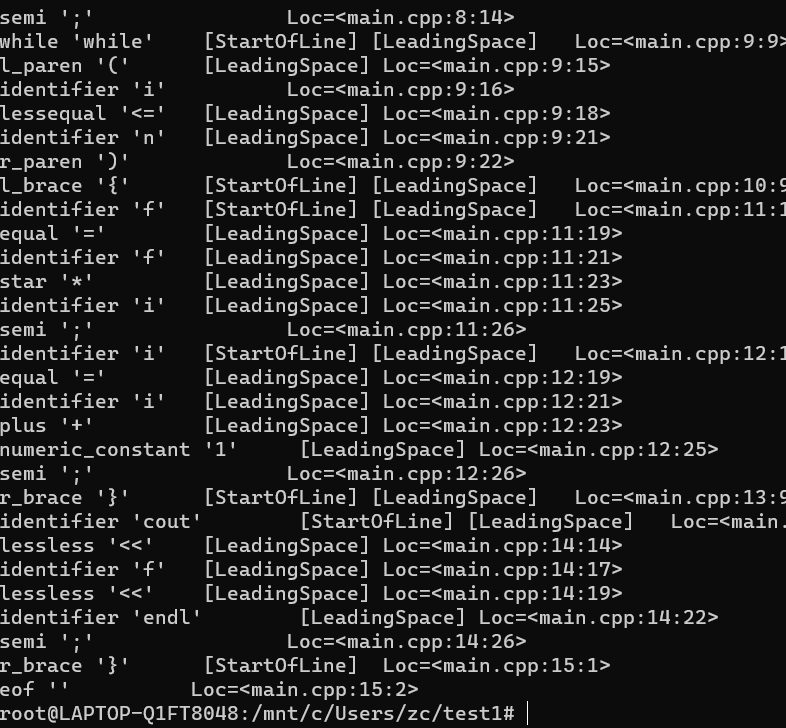
\includegraphics[width=0.5\textwidth,height=0.5\textwidth]{imgs/词法.png}
    \caption{词法分析}
    \label{fig:3}
\end{figure}
图\ref{fig:3}展示了一些词法单元的标识结果,并给出其属性和位置信息。

\paragraph{2.2 \ \ 语法分析}
在此阶段会将词法分析阶段产生的此法单元构建出抽象语法树。


LLVM 可以通过如下命令获得相应的 AST:
\begin{lstlisting}[frame=trbl]
  clang -E -Xclang -ast-dump main.cpp
\end{lstlisting}\par
结果如图\ref{fig:4}:
\begin{figure}[H]
    \centering
    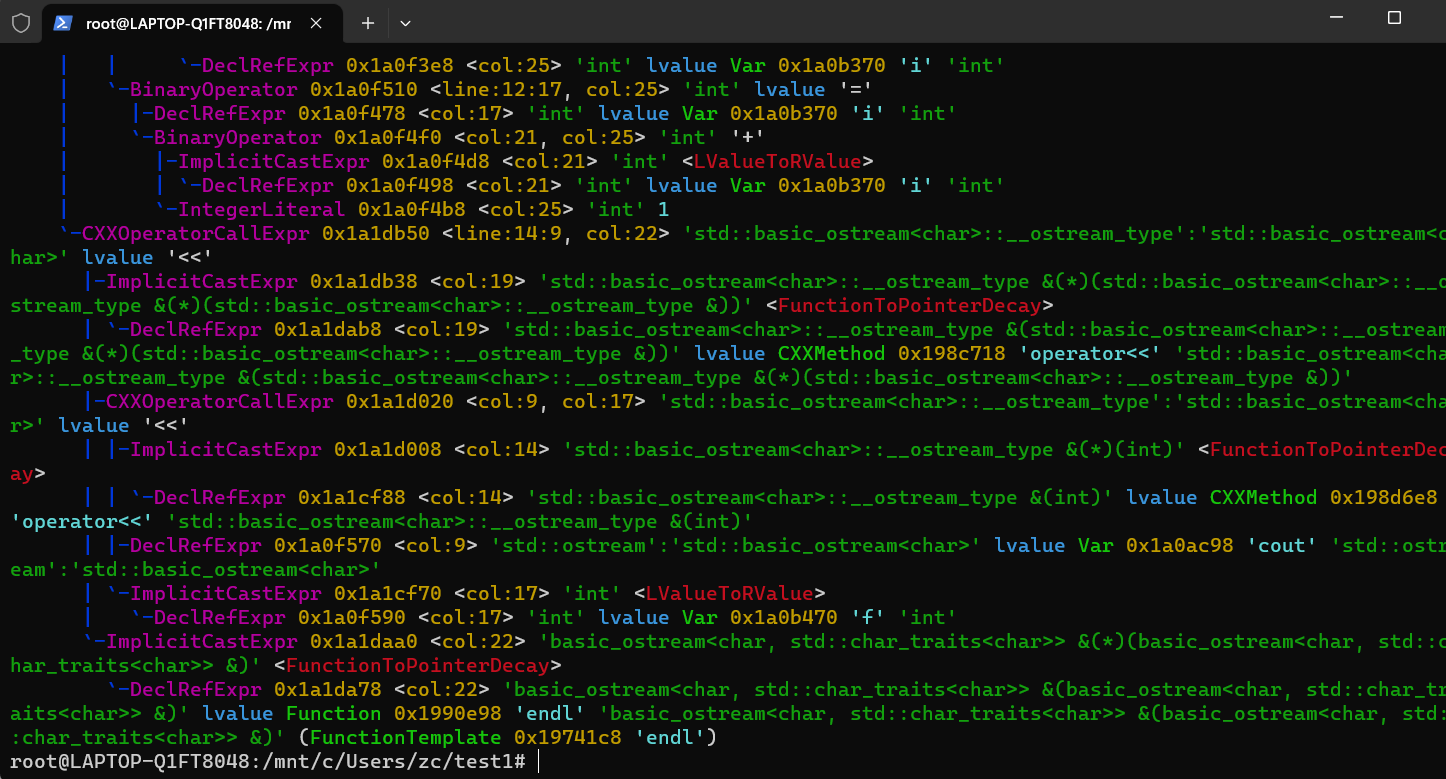
\includegraphics[width=0.7\textwidth,height=0.7\textwidth]{imgs/语法.png}
    \caption{语法单元标识结果}
    \label{fig:4}
\end{figure}

\paragraph{2.3 \ \ 语义分析}
使用语法树和符号表中信息来检查源程序是否与语言定义语义一致,进行类型检查等。

以下是语义分析阶段比较重要的部分:


类型检查。语义分析阶段会检查代码中的类型是否匹配,例如将整数值赋给浮点数变量、使用未声明的变量等。这有助于在编译过程中捕获一些常见的错误。


作用域分析。语义分析阶段会确定变量和标识符的可见范围,以及解析变量和函数的引用。这包括检查变量是否在正确的作用域内使用,以及解析函数调用的参数类型和返回类型。


常量折叠。语义分析阶段可能会对一些常量表达式进行求值,以便在后续的优化阶段中进行常量传播和折叠。


错误处理。语义分析阶段会检测并报告代码中的语义错误,例如重复定义的变量、函数调用参数不匹配等。编译器通常会生成有关错误的详细信息,以帮助开发人员定位和修复问题。


\paragraph{2.4 \ \ 中间代码生成}
编译器生成一个明确的低级或类机器语言的中间表示。


若想要可视化抽象语法树,以更好地分析代码依赖关系,可以先通过g++获得抽象语法树的.dot文件:
\begin{lstlisting}[frame=trbl]
  g++ -fdump-tree-all-graph main.cpp
\end{lstlisting}\par

结果如图\ref{fig:5}:
\begin{figure}[H]
    \centering
    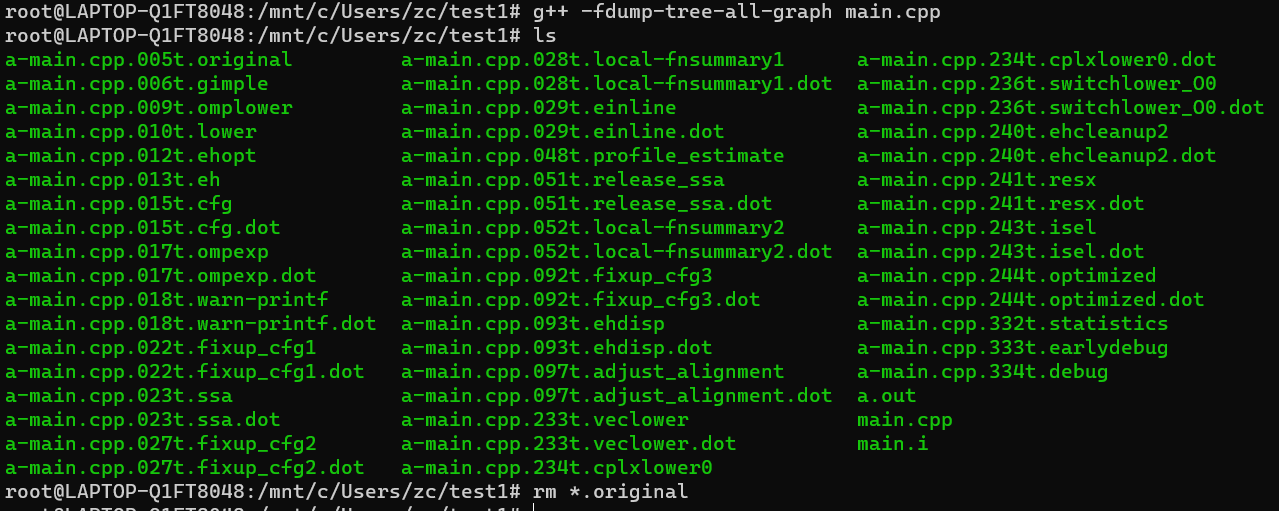
\includegraphics[width=0.7\textwidth,height=0.7\textwidth]{imgs/dot文件.png}
    \caption{所有.dot文件}
    \label{fig:5}
\end{figure}


使用 GraphViz可以为每个函数检索一个打印图(png文件),例如:
\begin{lstlisting}[frame=trbl]
  dot -Tpng a-main.cpp.015t.cfg.dot -o main.png
\end{lstlisting}\par
结果如图\ref{fig:6}:
\begin{figure}[H]
    \centering
    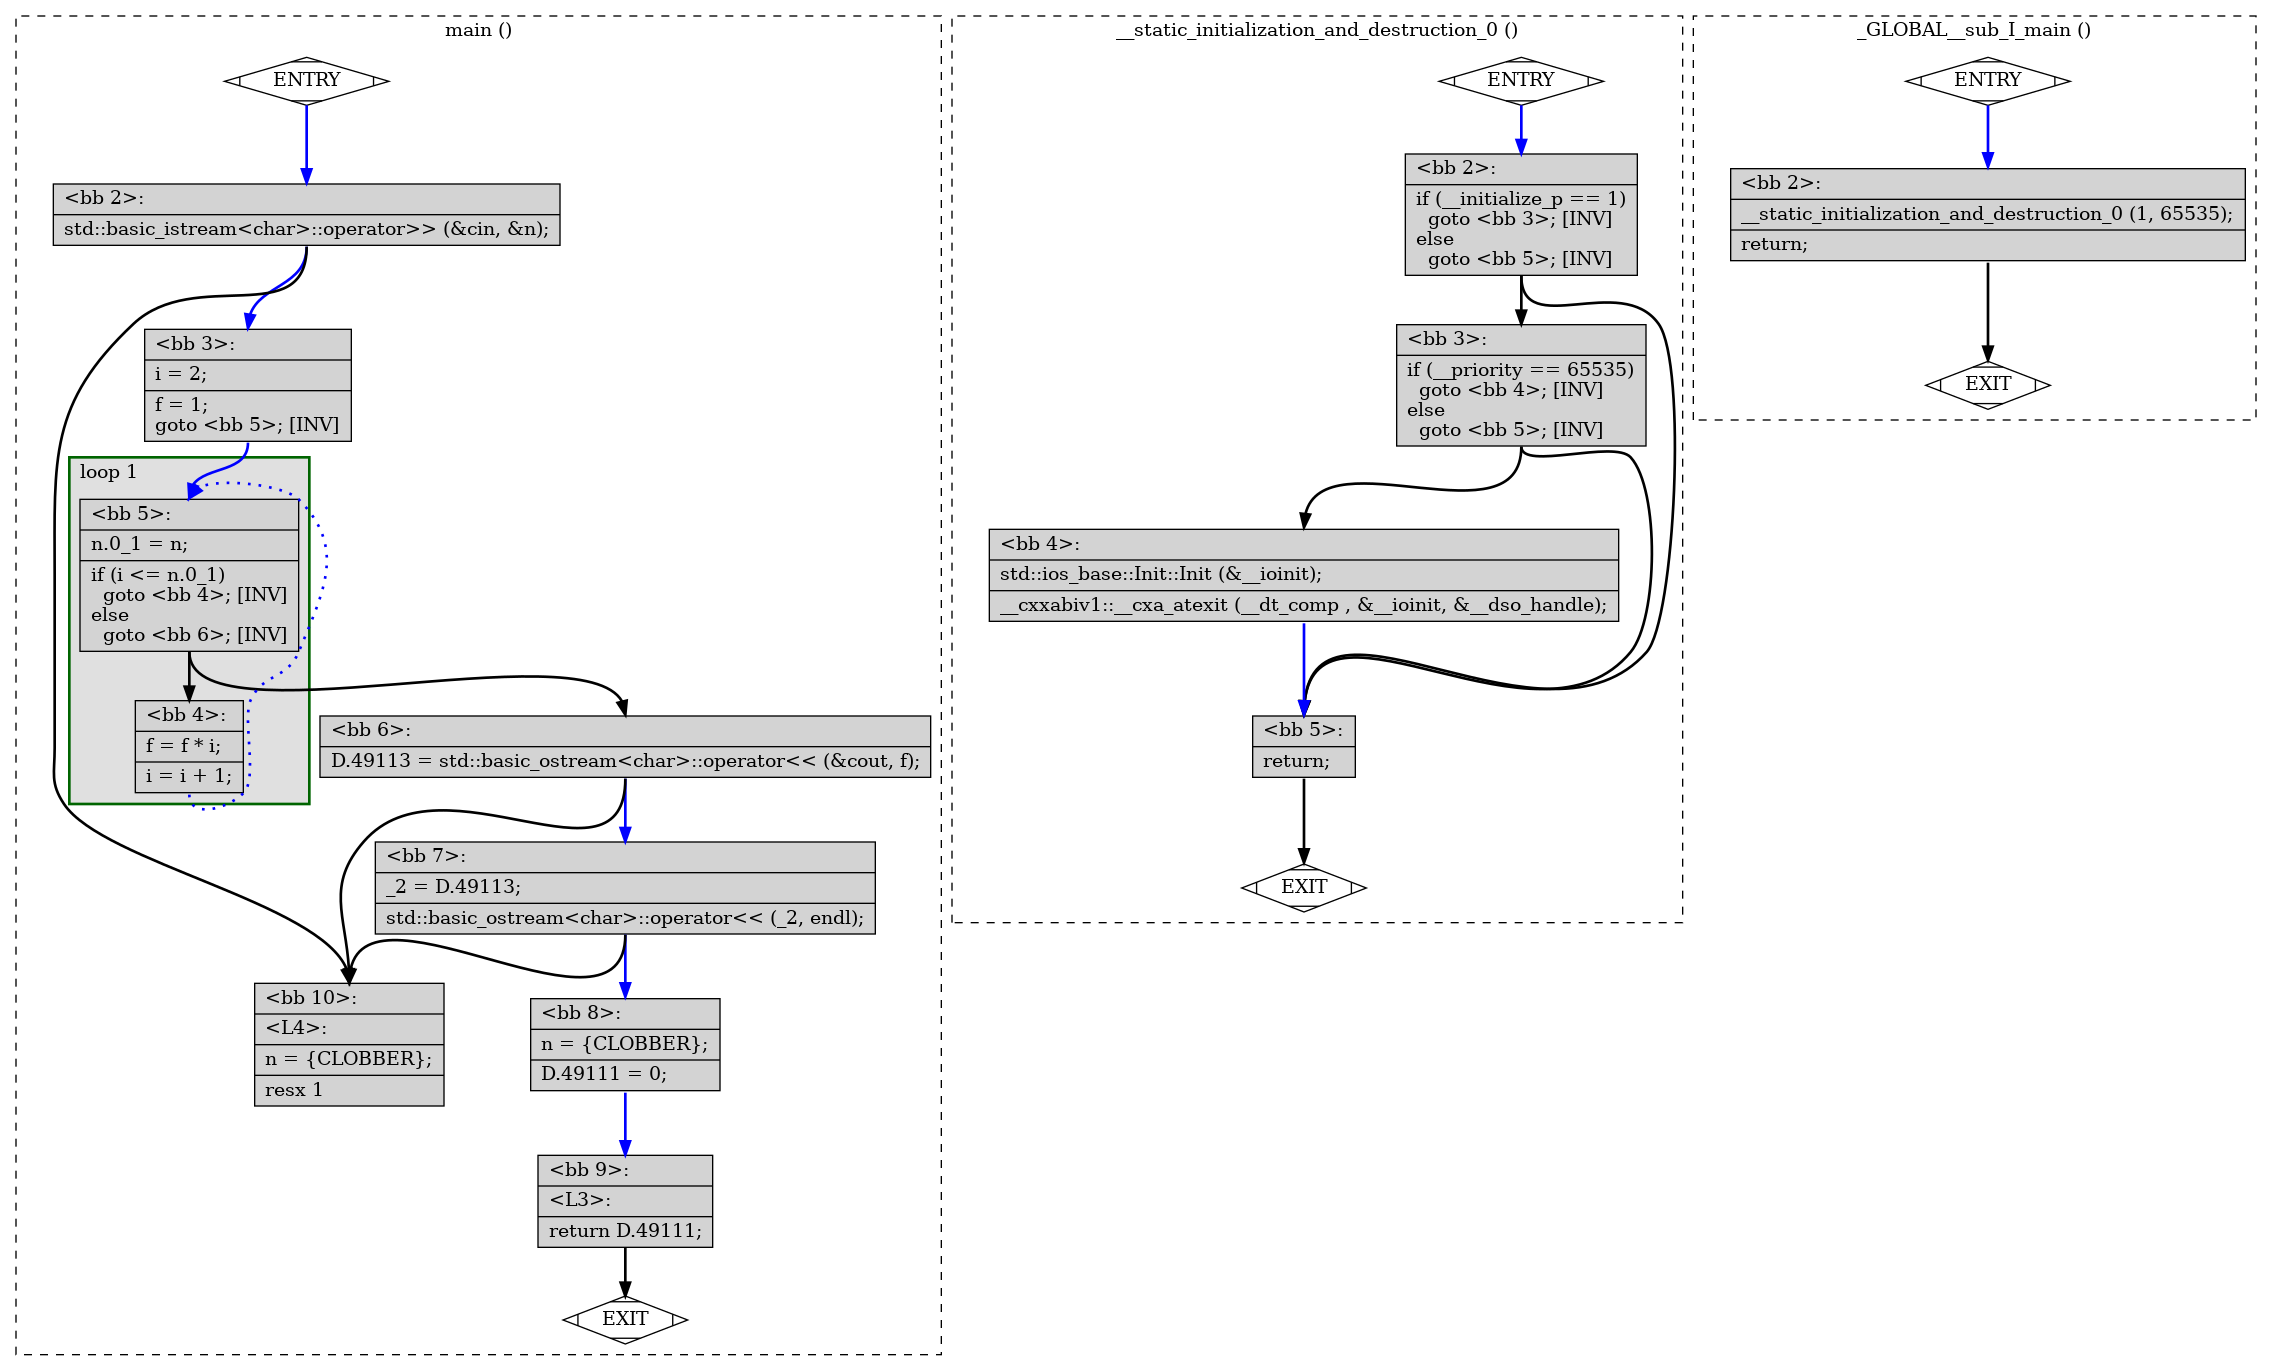
\includegraphics[width=0.8\textwidth,height=0.8\textwidth]{imgs/main.png}
    \caption{png文件}
    \label{fig:6}
\end{figure}


LLVM 可以通过下面的命令生成 LLVM IR:
\begin{lstlisting}[frame=trbl]
  clang -S -emit-llvm main.cpp
\end{lstlisting}\par
结果如图\ref{fig:7}:
\begin{figure}[H]
    \centering
    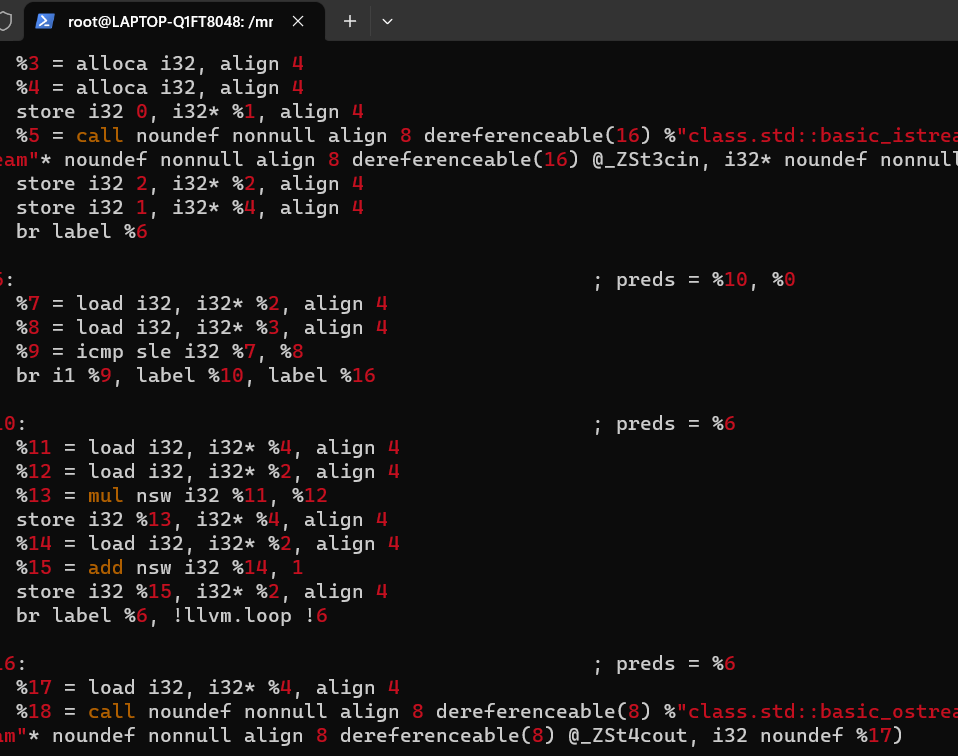
\includegraphics[width=0.6\textwidth,height=0.6\textwidth]{imgs/mainll.png}
    \caption{main.ll}
    \label{fig:7}
\end{figure}
LLVM IR 是LLVM编译器的中间表示形式,是一种类似汇编语言的表示形式,它包含了源代码的基本块、指令、变量和函数等信息,使得LLVM编译器可以对其进行各种优化和转换。


图\ref{fig:7}展示了一些函数声明和具体实现。

\paragraph{2.5 \ \ 代码优化}
进行与机器无关的代码优化步骤改进中间代码,生成更好的目标代码


通过命令:
\begin{lstlisting}[frame=trbl]
  llc -print-before-all -print-after-all main.ll > main.log 2>&1
\end{lstlisting}\par
将生成LLVM IR文件"main.ll"的编译过程中的调试输出,并将结果保存到"log"文件中。生成的"log"文件将包含LLC工具在编译LLVM IR文件期间的调试信息。这些信息可以用于分析和调试编译过程中的问题,如了解LLVM IR的转换和优化过程、查看生成的机器码等。


结果如图\ref{fig:8}:
\begin{figure}[H]
    \centering
    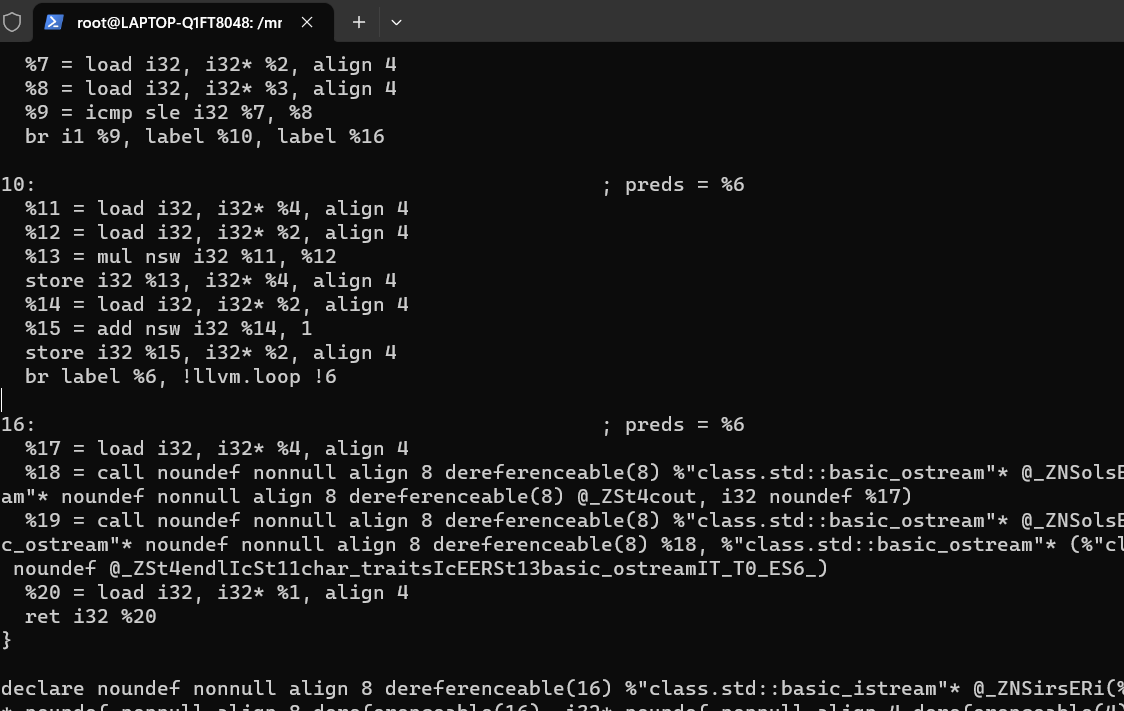
\includegraphics[width=0.7\textwidth,height=0.7\textwidth]{imgs/mainlog.png}
    \caption{main.log}
    \label{fig:8}
\end{figure}


可以通过命令:
\begin{lstlisting}[frame=trbl]
  llvm-as main.ll -o main.bc
  llvm-dis main.bc -o mian.ll
\end{lstlisting}\par
实现bc 和 ll 这两种 LLVM IR 格式的互转。


得到的main.bc如图\ref{fig:9}:
\begin{figure}[H]
    \centering
    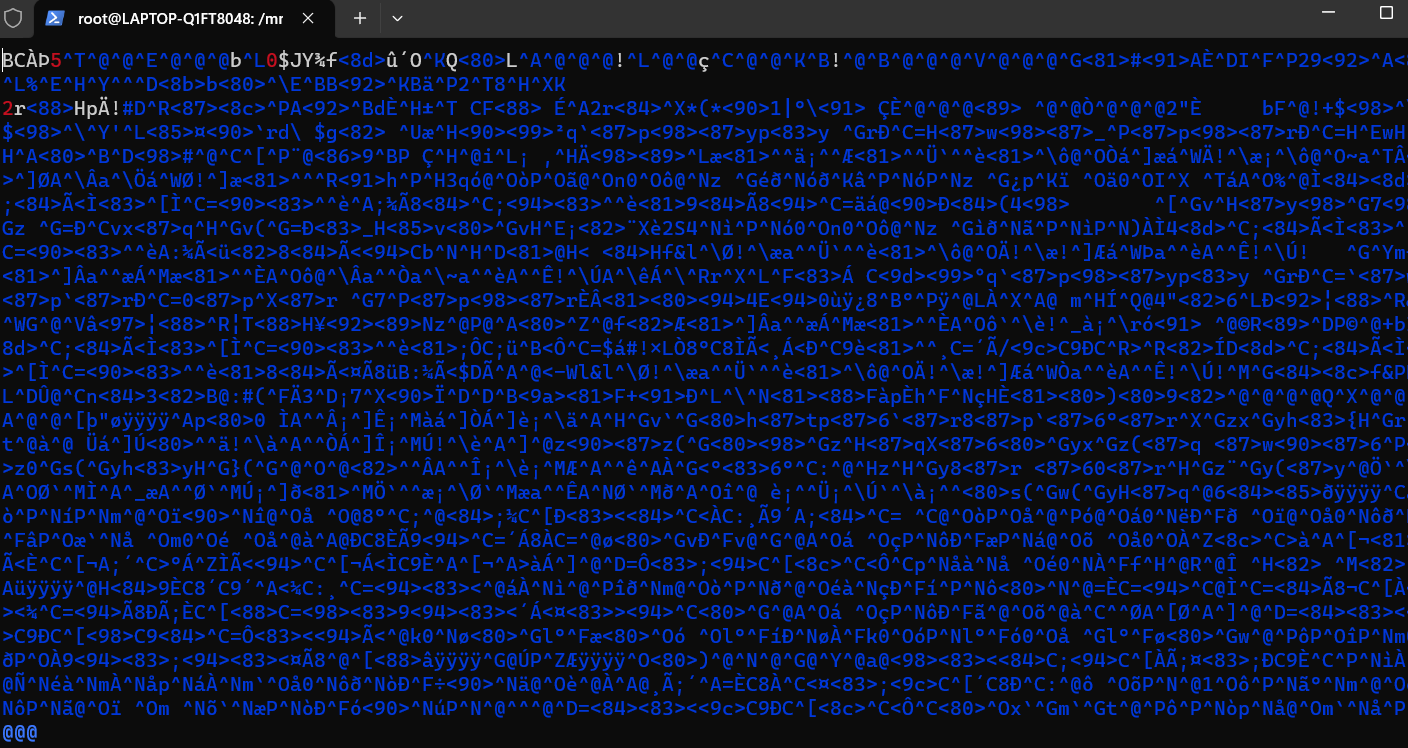
\includegraphics[width=0.7\textwidth,height=0.7\textwidth]{imgs/mainbc.png}
    \caption{main.bc}
    \label{fig:9}
\end{figure}

\paragraph{2.6 \ \ 代码生成}
以中间表示形式作为输入,将其映射到目标语言。


使用命令:
\begin{lstlisting}[frame=trbl]
  g++ -S -o main.S main.cpp
\end{lstlisting}\par
得到x86目标格式代码,如图\ref{fig:10}:
\begin{figure}[H]
    \centering
    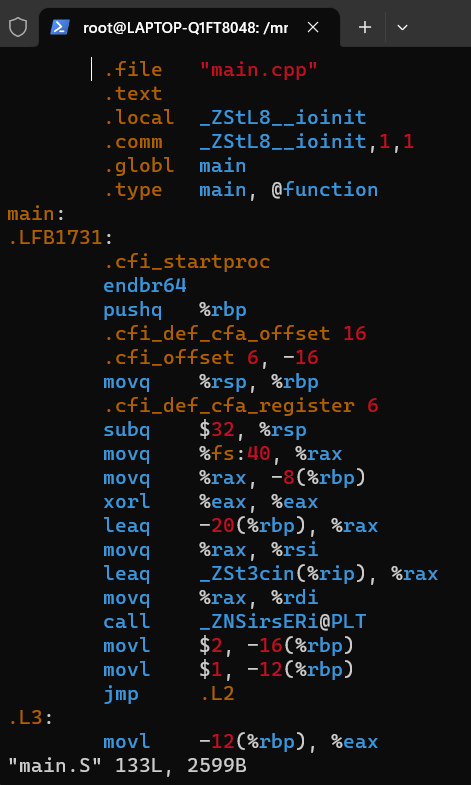
\includegraphics[width=0.6\textwidth,height=0.7\textwidth]{imgs/main_x86.png}
    \caption{main-x86.S}
    \label{fig:10}
\end{figure}


使用命令:
\begin{lstlisting}[frame=trbl]
  arm-linux-gnueabihf-g++ main.cpp -S -o main_arm.S
\end{lstlisting}\par
得到arm目标格式代码,如图\ref{fig:11}:
\begin{figure}[H]
    \centering
    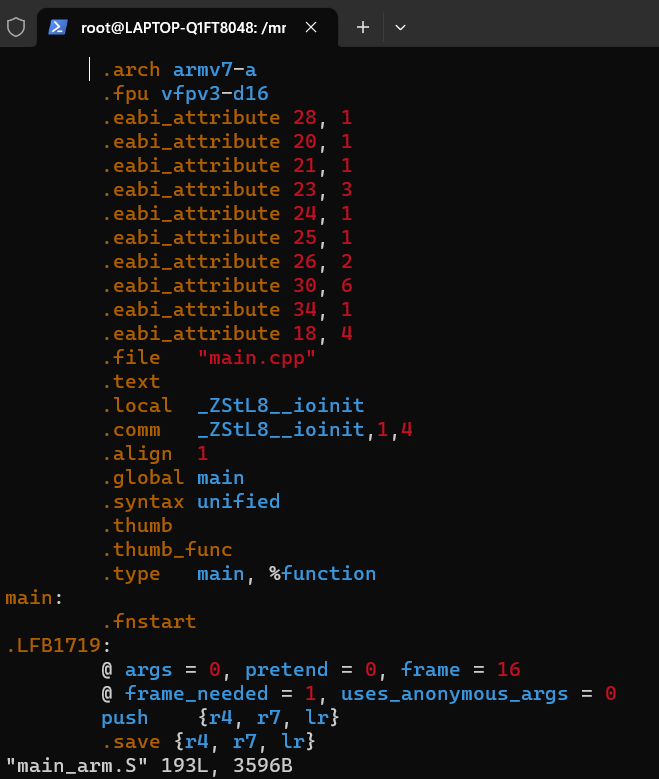
\includegraphics[width=0.6\textwidth,height=0.7\textwidth]{imgs/main_arm.png}
    \caption{main-arm.S}
    \label{fig:11}
\end{figure}

使用命令:
\begin{lstlisting}[frame=trbl]
  llc main.ll -o main.S
\end{lstlisting}\par
LLVM生成目标代码,如图\ref{fig:12}:
\begin{figure}[H]
    \centering
    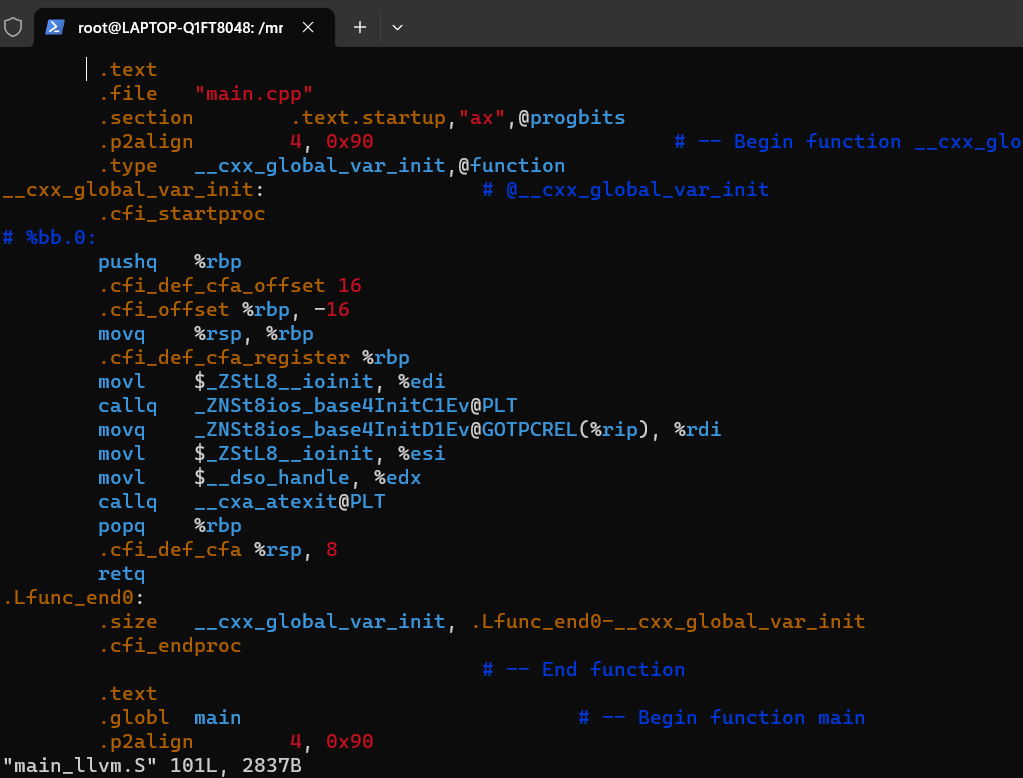
\includegraphics[width=0.6\textwidth,height=0.7\textwidth]{imgs/main_llvm.png}
    \caption{main-llvm.S}
    \label{fig:12}
\end{figure}
在代码生成阶段的x86、ARM和LLVM文件的区别主要体现在指令集架构、指令集、编译器平台、代码优化和性能功耗等方面。选择适合特定需求的目标平台和编译器平台,能获得最佳的性能和效率。



%——————————————————————————————————————
\subsection{第三节 \ \ 汇编器}
汇编器实现了从汇编语言翻译成目标机器指令的过程,最终生成的是可重定位的机器码。\par
在Linux终端上,通过以下命令得到生成的.o目标代码文件:
\begin{lstlisting}[frame=trbl]
  gcc -c jiechen.c -o  jiechen_x86.o
\end{lstlisting}\par
其中jiechen.c 和 jiechen\_x86.o是文件名\par
jiechen.c源代码如下:
\begin{lstlisting}[frame=trbl]
#include<stdio.h>
int main(){
    int i, n, f;
    scanf("%d",&n);
    i = 2;
    f = 1;
    while (i <= n) {
       f = f * i;
       i = i + 1;
    }
    printf("%d",f);
    return 0;
 }
\end{lstlisting}\par
通过objdump工具可以获得目标机器代码的相关内容,输入以下命令得到所有节(section)的信息:
\begin{lstlisting}[frame=trbl]
  objdump -h jiechen_x86.o
\end{lstlisting}\par
得到如下结果:
\begin{lstlisting}[frame=trbl]
  jiechen_x86.o:     文件格式 elf64-x86-64

节:
Idx Name          Size      VMA               LMA             File off  Algn
0 .text         00000090  0000000000000000  0000000000000000  00000040  2**0
                  CONTENTS, ALLOC, LOAD, RELOC, READONLY, CODE
1 .data         00000000  0000000000000000  0000000000000000  000000d0  2**0
                  CONTENTS, ALLOC, LOAD, DATA
2 .bss          00000000  0000000000000000  0000000000000000  000000d0  2**0
                  ALLOC
3 .rodata       00000003  0000000000000000  0000000000000000  000000d0  2**0
                  CONTENTS, ALLOC, LOAD, READONLY, DATA
4 .comment      0000002c  0000000000000000  0000000000000000  000000d3  2**0
                  CONTENTS, READONLY
5 .note.GNU-stack 00000000  0000000000000000  0000000000000000  000000ff  2**0
                  CONTENTS, READONLY
6 .note.gnu.property 00000020  0000000000000000  0000000000000000  00000100  2**3
                  CONTENTS, ALLOC, LOAD, READONLY, DATA
7 .eh_frame     00000038  0000000000000000  0000000000000000  00000120  2**3
                  CONTENTS, ALLOC, LOAD, RELOC, READONLY, DATA
\end{lstlisting}\par
字段具体含义:\par
Idx:节的索引号\par
Name:节的名称\par
Size:节的大小(以字节为单位)\par
VMA (Virtual Memory Address):节在虚拟内存中的地址\par
LMA (Load Memory Address):节在链接时的内存地址\par
File off:节在文件中的偏移量(以字节为单位)\par
Algn:节的对齐方式\par
CONTENTS,ALLOC,LOAD等为每一个节所具有的属性.节具体含义:\par
.text:保存程序的可执行指令代码,即程序的代码区\par
.data:存储程序的初始化全局变量和静态变量\par
.bss:存储程序的未初始化全局变量和静态变量\par
.rodata:包含了程序的只读数据,如字符串常量\par
.comment:包含了一些编译器的元数据或注释信息\par
.note.GNU-stack:含有关于目标文件堆栈的特性的信息,例如是否堆栈是可执行的。\par
.note.gnu.property:包含了一些GNU特有的属性信息\par
.eh\_frame:包含了用于异常处理的信息。\par
由实验结果可以看到,由于i,n,f等变量声明在main函数中,属于局部变量,保存在栈区,故源程序未声明全局变量,data节和bss节大小为0字节。
下面尝试在源代码中声明全局变量和常量,重新生成目标代码文件,观察上述三节大小是否变化\par
对代码(jiechen.c)进行修改:
\begin{lstlisting}[title=阶乘,frame=trbl,language={C++}]
#include<stdio.h>
char b ;
int c = 1122;
const int a = 0 ;
int main(){
    int i, n, f;
    scanf("%d",&n);
    i = 2;
    f = 1;
    while (i <= n) {
       f = f * i;
       i = i + 1;
    }
    printf("%d",f);
    return 0;
 }
\end{lstlisting}
然后通过objdump重新查看.bss、.data和.rodata节的相关信息:
\begin{lstlisting}[frame=trbl]
Idx Name          Size      VMA               LMA             File off  Algn
1 .data         00000004  0000000000000000  0000000000000000  000000d0  2**0
                  CONTENTS, ALLOC, LOAD, DATA
2 .bss          00000001  0000000000000000  0000000000000000  000000d0  2**0
                  ALLOC
3 .rodata       00000007  0000000000000000  0000000000000000  000000d0  2**0
                  CONTENTS, ALLOC, LOAD, READONLY, DATA
\end{lstlisting}\par
可以看到,声明的字符型变量b为全局变量,且未完成初始化,故分配在bss节中,该节的大小变为0x00000001,而
整形常量a初始化为0,分配在rodata节中,该节的大小变为0x00000007,在原有基础上增加4字节,整形变量c初始化为0,分配在data节,data节增加4字节,符合实验预期。\par
同时从实验结果看到,所有节的VMA此时均为0,这是由于目标文件还没有被链接。在链接阶段,链接器会将所有的目标文件和库文件合并到一个单一的可执行文件或库文件中,为每个节分配适当的地址。此时每个节在最终的可执行文件中会有一个唯一的非零的虚拟内存地址。\\
\\
\\
% 参考文献\cite{adams1995hitchhiker}\cite{shin2016deep}
  % 备忘:  jiechen\_x86\_new是.c生成的
  %   jiechen\_x86是有.S生成的




\subsection{第四节 \ \ 链接器}
链接器(linker)负责将多个编译产生的对象文件(object files)和库(libraries)合并成一个单一的可执行文件(executable file)或库文件。通过以下命令将目标代码文件链接成可执行文件(ELF):
\begin{lstlisting}[frame=trbl]
gcc -o jiechen_x86 jiechen_x86.o
\end{lstlisting}\par
然后在终端打开可执行文件,键入阶乘数字4,得到结果24,说明该文件成功正确执行。再通过objdump查看文件节的相关信息(只截取15-26节信息):
\begin{lstlisting}[frame=trbl]
Idx Name          Size      VMA               LMA             File off  Algn
15 .text         00000179  00000000000010a0  00000000000010a0  000010a0  2**4
                  CONTENTS, ALLOC, LOAD, READONLY, CODE
16 .fini         0000000d  000000000000121c  000000000000121c  0000121c  2**2
                  CONTENTS, ALLOC, LOAD, READONLY, CODE
17 .rodata       00000007  0000000000002000  0000000000002000  00002000  2**2
                  CONTENTS, ALLOC, LOAD, READONLY, DATA
18 .eh_frame_hdr 00000034  0000000000002008  0000000000002008  00002008  2**2
                  CONTENTS, ALLOC, LOAD, READONLY, DATA
19 .eh_frame     000000ac  0000000000002040  0000000000002040  00002040  2**3
                  CONTENTS, ALLOC, LOAD, READONLY, D1ATA
20 .init_array   00000008  0000000000003da8  0000000000003da8  00002da8  2**3
                  CONTENTS, ALLOC, LOAD, DATA
21 .fini_array   00000008  0000000000003db0  0000000000003db0  00002db0  2**3
                  CONTENTS, ALLOC, LOAD, DATA
22 .dynamic      000001f0  0000000000003db8  0000000000003db8  00002db8  2**3
                  CONTENTS, ALLOC, LOAD, DATA
23 .got          00000058  0000000000003fa8  0000000000003fa8  00002fa8  2**3
                  CONTENTS, ALLOC, LOAD, DATA
24 .data         00000010  0000000000004000  0000000000004000  00003000  2**3
                  CONTENTS, ALLOC, LOAD, DATA
25 .bss          00000008  0000000000004010  0000000000004010  00003010  2**0
                  ALLOC
26 .comment      0000002b  0000000000000000  0000000000000000  00003010  2**0
                  CONTENTS, READONLY
\end{lstlisting}\par
此时发现VMA已经非0,为实际虚拟内存地址。这是因为在链接过程中完成了代码重定位。链接器修改目标文件中的代码和数据,使其对应于分配的地址。其中包括更新指令和数据中的地址引用,以使它们指向正确的位置。确定地址:确定每个符号(如函数和全局变量)在最终程序中的实际地址;更新地址引用:更新代码和数据段中的所有地址引用,使其指向正确的实际地址。\par
同时发现可执行文件相较于.o目标代码文件,节的数量有所增加。部分节(如text和data)的大小也增加了。这是因为,运行和启动代码时,为了使程序能够运行,链接器会添加一些额外的代码和数据。这会增加新的节和增加现有节的大小。如:gnu.version节存储版本控制的相关信息。init节中存储程序初始化代码。通过以下命令查看可执行文件的反汇编代码:
\begin{lstlisting}[frame=trbl]
objdump -d jiechen_x86
\end{lstlisting}\par
截取以下内容:
\begin{lstlisting}[frame=trbl]
0000000000001000 <_init>:
00000000000010a0 <_start>:
    10a0:	f3 0f 1e fa          	endbr64 
    10a4:	31 ed                	xor    %ebp,%ebp
    10a6:	49 89 d1             	mov    %rdx,%r9
    10a9:	5e                   	pop    %rsi
    10aa:	48 89 e2             	mov    %rsp,%rdx
    10ad:	48 83 e4 f0          	and    $0xfffffffffffffff0,%rsp
    10b1:	50                   	push   %rax
    10b2:	54                   	push   %rsp
    10b3:	45 31 c0             	xor    %r8d,%r8d
    10b6:	31 c9                	xor    %ecx,%ecx
    10b8:	48 8d 3d ca 00 00 00 	lea    0xca(%rip),%rdi        # 1189 <main>
    10bf:	ff 15 13 2f 00 00    	call   *0x2f13(%rip)        
                                        # 3df8<__libc_start_main@GLIBC_2.34>
    10c5:	f4                   	hlt    
    10c6:	66 2e 0f 1f 84 00 00 	cs nopw 0x0(%rax,%rax,1)
    10cd:	00 00 00 
0000000000001189 <main>:
  # …… 中间代码省略
1218:	c3                   	ret    # <main>函数结束地址
\end{lstlisting}\par
程序执行流程:由上可以看到,程序最开始执行init节中的代码,完成程序启动前的初始化。然后进入0x10a0,即Entry Point执行启动函数,启动函数最后会调用main函数,从而开始执行main函数内容。\par
同时,程序调用动态链接库时,会用dynamic节保存相关信息。如果是多个.o文件一起链接成可执行文件,链接器还会将text这样的节合并成一个更大的text节。如果多个.o文件中存在符号引用,即解析在一个对象文件中定义而在另一个对象文件中引用的符号(如函数或全局变量)。ELF文件的首部有ELF文件头(类似于Windows系统下的PE文件头),用于描述文件的总体信息,如:版本,文件类型,机器类型等。\par
再通过objdump反汇编jiechen\_x86.o发现,反汇编代码中只有<main>内容,且大小为0x8f,刚好等于可执行文件中<main>的大小:0x1218 -0x1189=0x8f,同时反汇编代码未发生改变,即说明链接过程中main函数大小和内容未改变。链接实质上是将目标文件、版本信息、程序初始化内容、链接加载动态链接库和文件头等封装在了一起。\\
\\
\\



\subsection{第五节 \ \ LLVM编程}
下面对斐波拉契数列程序尝试使用LLVM 中间语言来实现。直接编写较为困难,结合.c编译出的.ll文件一起理解。
\begin{lstlisting}[frame=trbl]
define dso_local i32 @main() #0 {
  ;需要声明5个变量,同时需要一个恒为0的寄存器,故一共声明6个虚拟寄存器
  %1 = alloca i32, align 4    ;为%1变量分配32bit的空间
  %2 = alloca i32, align 4    ;声明int a
  %3 = alloca i32, align 4    ;声明int b
  %4 = alloca i32, align 4    ;声明int i
  %5 = alloca i32, align 4    ;声明int t
  %6 = alloca i32, align 4    ;声明int n
  store i32 0, i32* %1, align 4      ;恒0寄存器
  store i32 0, i32* %2, align 4      ;a=0
  store i32 1, i32* %3, align 4      ;b=1
  store i32 1, i32* %4, align 4      ;i=1
  
  ;调用scanf函数,第二个参数即为%6,即变量n
  %7 = call i32 (i8*, ...) @__isoc99_scanf(i8* noundef getelementptr inbounds ([3 x i8], [3 x i8]* @.str, i64 0, i64 0), i32* noundef %6)
  
  ;为下一步printf做准备
  %8 = load i32, i32* %3, align 4
  ;调用printf
  %9 = call i32 (i8*, ...) @printf(i8* noundef getelementptr inbounds ([4 x i8], [4 x i8]* @.str.1, i64 0, i64 0), i32 noundef %8)
  br label %10   ;无条件跳转到%10

;%10对应while循环的条件判断
10:                                               ; preds = %14, %0
  %11 = load i32, i32* %4, align 4     ;将i加载到内存中
  %12 = load i32, i32* %6, align 4     ;将n加载到内存中
  %13 = icmp slt i32 %11, %12          ;用%13保存比较的布尔值
  br i1 %13, label %14, label %24      ;有条件跳转

;循环体
14:                                               ; preds = %10
  ;对应t=b
  %15 = load i32, i32* %3, align 4    
  store i32 %15, i32* %5, align 4
  
  ;对应b=a+b
  %16 = load i32, i32* %2, align 4
  %17 = load i32, i32* %3, align 4
  %18 = add nsw i32 %16, %17          ;存储加法结果后store回变量b中
  store i32 %18, i32* %3, align 4

  ;对应printf("%d\n",b);
  %19 = load i32, i32* %3, align 4
  %20 = call i32 (i8*, ...) @printf(i8* noundef getelementptr inbounds ([4 x i8], [4 x i8]* @.str.1, i64 0, i64 0), i32 noundef %19)

  ;对应a=t
  %21 = load i32, i32* %5, align 4
  store i32 %21, i32* %2, align 4

  ;对应i=i+1
  %22 = load i32, i32* %4, align 4
  %23 = add nsw i32 %22, 1
  store i32 %23, i32* %4, align 4
  
  br label %10, !llvm.loop !6    ;无条件跳转,回到while的判断部分

24:                                               ; preds = %10
  ret i32 0    ;return 0
}
\end{lstlisting}\par
采用以下命令,通过LLVM将.ll程序编译成目标程序,进而链接成可执行文件:
\begin{lstlisting}[frame=trbl]
llvm-as fib.ll -o fib.bc             # 采用二进制形式
llc fib.bc  -filetype=obj -o fib.o   # 将LLVM编译成目标代码文件
gcc -o fib fib.o                     # 将目标文件链接成可执行文件 
\end{lstlisting}\par
打开fib后,输入数字5,得到1,1,2,3,5序列。说明程序正确执行。
\newpage
\bibliographystyle{plain}
\bibliography{references} 
\end{document}
